\section{Product perspective}
\label{sec:product_perspesctive}%

\subsection{Scenarios}
\label{subsec:scenarios}%

\paragraph{Scenario 1: Giovanni Joins S\&C to Begin His Internship Search}

Giovanni, a university student, is looking to gain some practical
experience through an internship. He's aware that securing a good
internship is crucial for his future career, but he
doesn't know where to begin his search. One evening,
while discussing internship opportunities with his friends, Giovanni
hears about the S\&C platform, which helps match students with
internships based on their CVs and company needs. Intrigued, he decides
to download the application.

During the sign-up process, Giovanni provides the required information:
his email, password, first name, last name and username. Once his
account is created, he logs in and completes his profile. With
everything set up, Giovanni is ready to explore the various internship
opportunities available to him on the platform.


\paragraph{Scenario 2: Zoogle Joins S\&C to Find Talented Interns}

Zoogle, a growing tech company, is on the lookout for talented students
to join its internship program. The company values fresh ideas and
practical skills and believes that collaborating with university
students can bring innovation to its projects.

After hearing about the S\&C platform, which connects companies with
university students seeking internships, Zoogle decides to join. A
representative from the company creates an account by providing the
necessary information: the company's email, name, VAT number and username.
Once the registration is complete, Zoogle gains access to the platform.


\paragraph{Scenario 3: Zoogle Creates an Internship Posting on S\&C}

Zoogle is ready to recruit university students for its internship
program. The HR team at Zoogle logs into the S\&C platform to post a new
internship position.

They fill out the internship posting form with all the necessary
details: the Internship Title, Description, Required Skills, Duration,
Location, and Eligibility Criteria. Once the details are submitted, the
position becomes available to thousands of students seeking
opportunities. With the new internship posting live, Zoogle is eager to connect with
talented candidates like Giovanni.


\paragraph{Scenario 4: Giovanni Navigates Suggested Companies and Applies for an Internship}

Giovanni, eager to find the right internship, navigates through the
suggested companies on his S\&C homepage. These recommendations are
generated by the system based on his experience, skills and interests.

As he explores the suggestions, Giovanni discovers an internship
opportunity at Zoogle. He reviews the position and finds that it matches
his qualifications perfectly. Excited, Giovanni clicks on the
opportunity, begins the application process and submits his application
to Zoogle.


\paragraph{Scenario 5: Giovanni Provides Feedback on a Recommended
Internship}

After Giovanni reviewed the suggested internship at Zoogle and went back
to the Homepage, a pop-up appears asking him for feedback on the
recommendation. The system inquires whether the recommendation was
useful, and Giovanni is prompted to provide a rating and a comment.

Giovanni, feeling that the suggestion matches his interests and
qualifications, selects that the recommendation was useful and provides
some positive rating and feedback. His input helps the
system's statistical analysis engine, which uses this
data to enhance future internship recommendations for other students
based on skills, interests, CVs, and other factors.


\paragraph{Scenario 6: Zoogle Reviews and Selects Student CVs}

Zoogle's HR team wants to find the right candidate for their internship
position, so they log in to the S\&C platform. Upon logging in, they
access to his profile page and after clicking on one of their insertion,
two candidate's lists appears: the list of students who have applied to their
internship and the list of students whose profiles have been recommended to them by
the system, based on qualifications, experience, and preferences.

The HR team first goes through the list of students who applied for the
internship. After reviewing the CVs, Zoogle's HR representatives select
Giovanni's profile from that list, creating a contact. A chat is opened,
allowing Giovanni and Zoogle to communicate directly and proceed to the
next steps in the hiring process.


\paragraph{Scenario 7: Giovanni and Zoogle Schedule an Interview}

After the contact is established between Giovanni and Zoogle, they
begin communicating through the chat feature on the S\&C platform.
Zoogle's HR team proposes scheduling an interview, and
Giovanni agrees. The interview is then scheduled on the S\&C
calendar, and takes place outside the S\&C platform, using a
video conferencing tool or in person, depending on the company's
preference.

After the interview's scheduling, both parties prepare for the next step
in the hiring process, moving closer to a potential internship offer.


\paragraph{Scenario 8: Zoogle Offers Giovanni an Internship Position}

After conducting the interview with Giovanni, Zoogle's HR team is
impressed by his skills, enthusiasm, and alignment with the company's
values. Giovanni, in turn, felt a strong connection with the team and
was excited about the role and responsibilities. Both Giovanni and
Zoogle's HR team recognized a great mutual fit.

Given their positive impressions of each other, Zoogle's HR team
proposes Giovanni the internship contract he applied for. Giovanni
agrees on the contract's conditions and accepts the proposal through the
chat.


\paragraph{Scenario 9: Giovanni Submits a Complaint About His Internship
and PoliCt decides to interrupt his internship}

Giovanni has started his internship at Zoogle, but he encounters a
problem that affects his experience. Unsatisfied with certain aspects of
the internship, he decides to raise the issue through the S\&C platform.

Giovanni logs into his profile, clicks chat section, enters into the
chat and submit a complaint.

PoliCt, Giovanni's university, which monitors the internship program
through the S\&C platform, reviews Giovanni's complaint.
After evaluating the situation, PoliCt decides to act and
interrupts Giovanni's internship with Zoogle.


\subsection{Class diagrams}
\label{subsec:class_diagrams}%


\begin{figure}[H]
    \begin{center}
        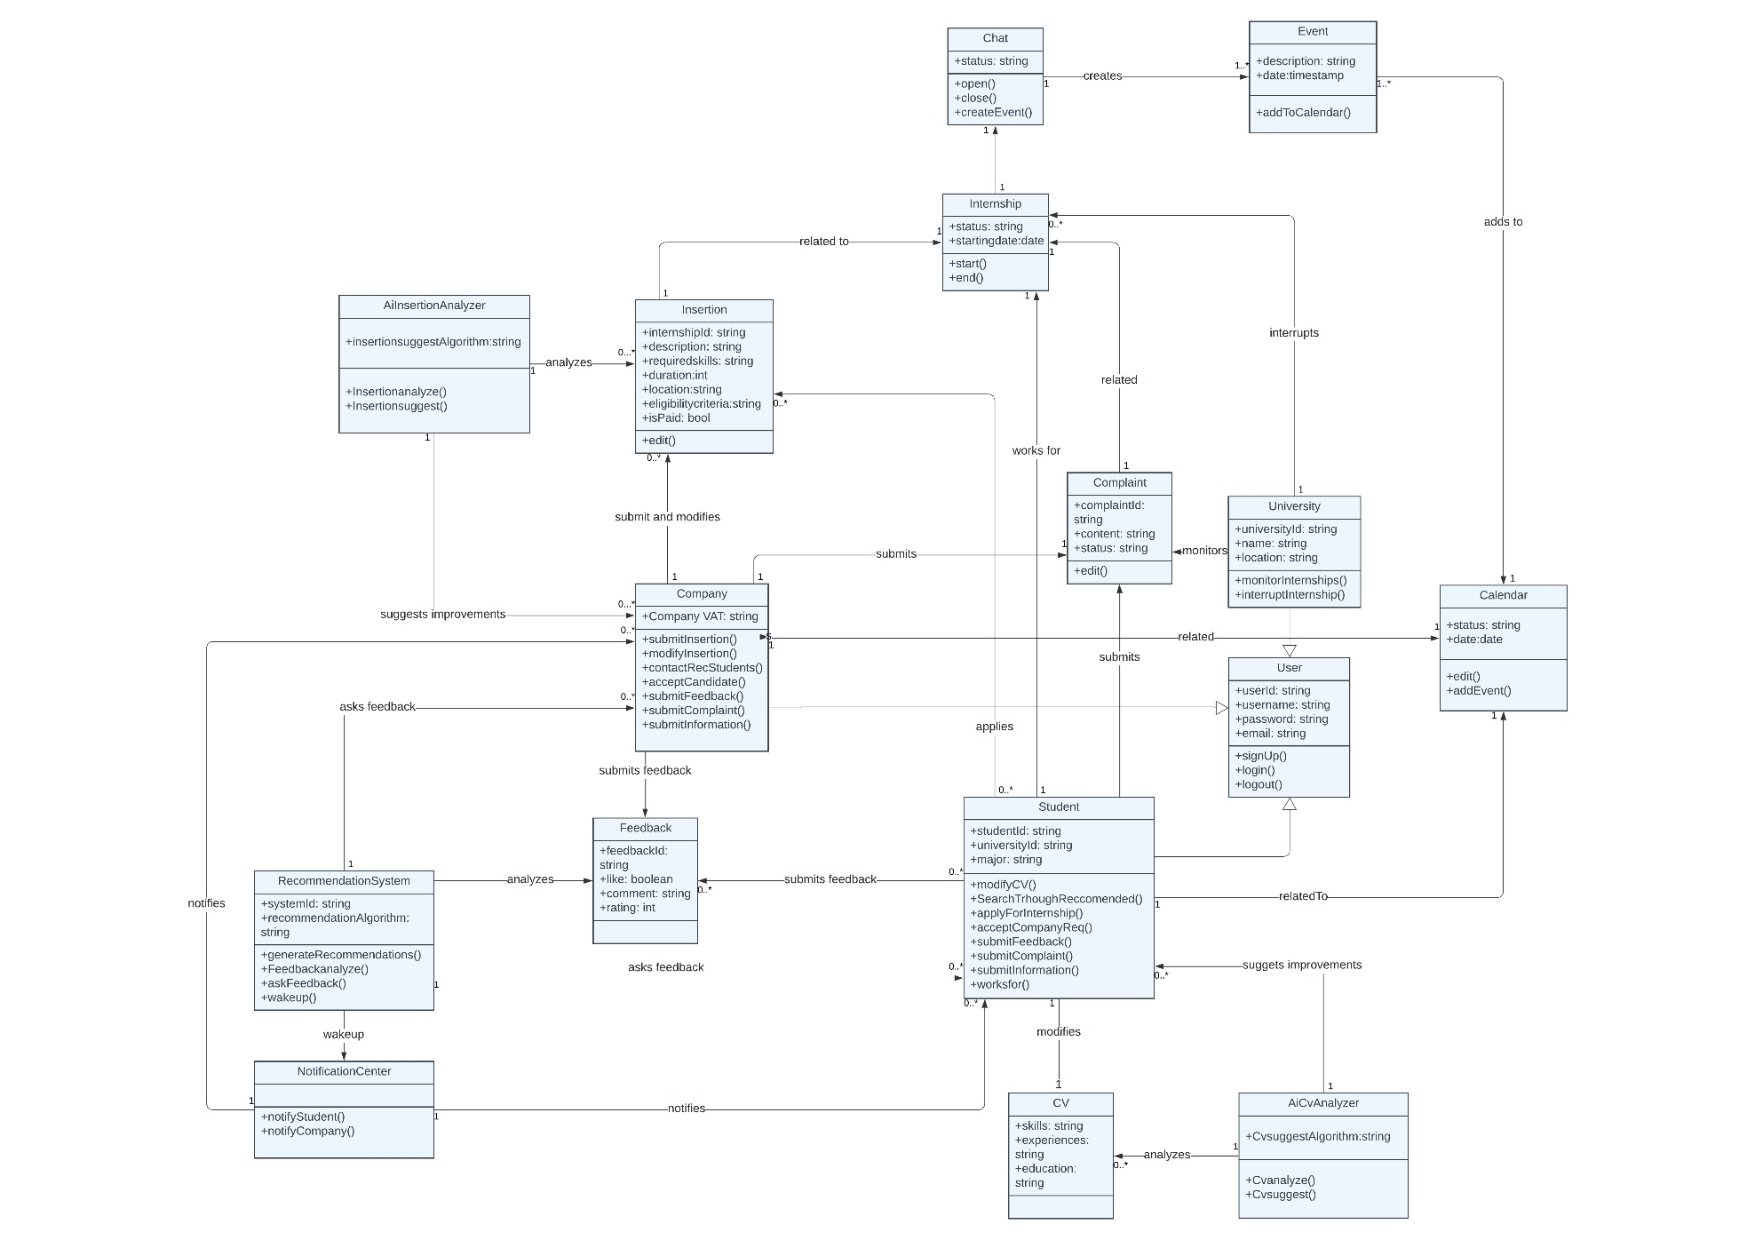
\includegraphics[width=\linewidth]{Images/ClassDiagram/UMLClass.pdf}
        \caption{UML Class Diagram.}
        \label{fig:UML_class_diag}%
    \end{center}
\end{figure}


The Student and Company classes extend the abstract class User. Companies can create and modify Insertion instances representing internship opportunities, which are analyzed using the AiInsertionAnalyzer class to provide recommendations.

The RecommendationSystem generates fitted recommendations for students based on their CV details, analyzed by the AiCVAnalyzer. Complaints and feedback are handled through the Complaint and Feedback classes, respectively, and notifications are sent using the NotificationCenter. Additionally, the University class oversees internships, with functionalities to monitor or interrupt them if necessary, while Calendar and Event classes manage scheduling activities like interviews and internship start dates.


\subsection{State diagrams}
\label{subsec:state_diagrams}%

In this section are presented the State Diagrams of the S\&C system
representing all the possible operation that a User can perform.

\paragraph{Sign Up:} The registration process on the S\&C platform begins
  when a new guest decides to create an account. If you represent a
  university, click on the "Are you a
  University?" button to begin the tailored
  registration process. Alternatively, upon selecting the "Sign up"
  option, the guest is prompted to choose between a student or company
  account. Depending on their selection, the system tailors the
  registration flow to gather specific information. After the
  registration form, the system performs a check on the credentials
  provided. It ensures that the email or nickname is not already in use
  by another user and verifies that the password meets the platform's
  security criteria: it must be at least 8 characters long, contain at
  least one capital letter, one number, and a special character. If any
  of these conditions are not met, the user receives an error message
  prompting them to adjust their input. Once the credentials are
  validated, the system prompts all users to verify their email
  addresses by sending a verification link to the email provided during
  registration. The guest must click this link to confirm their email,
  ensuring that the contact information is valid. Upon successful email
  verification, users are directed to complete their profile.

\begin{figure}[H]
    \begin{center}
        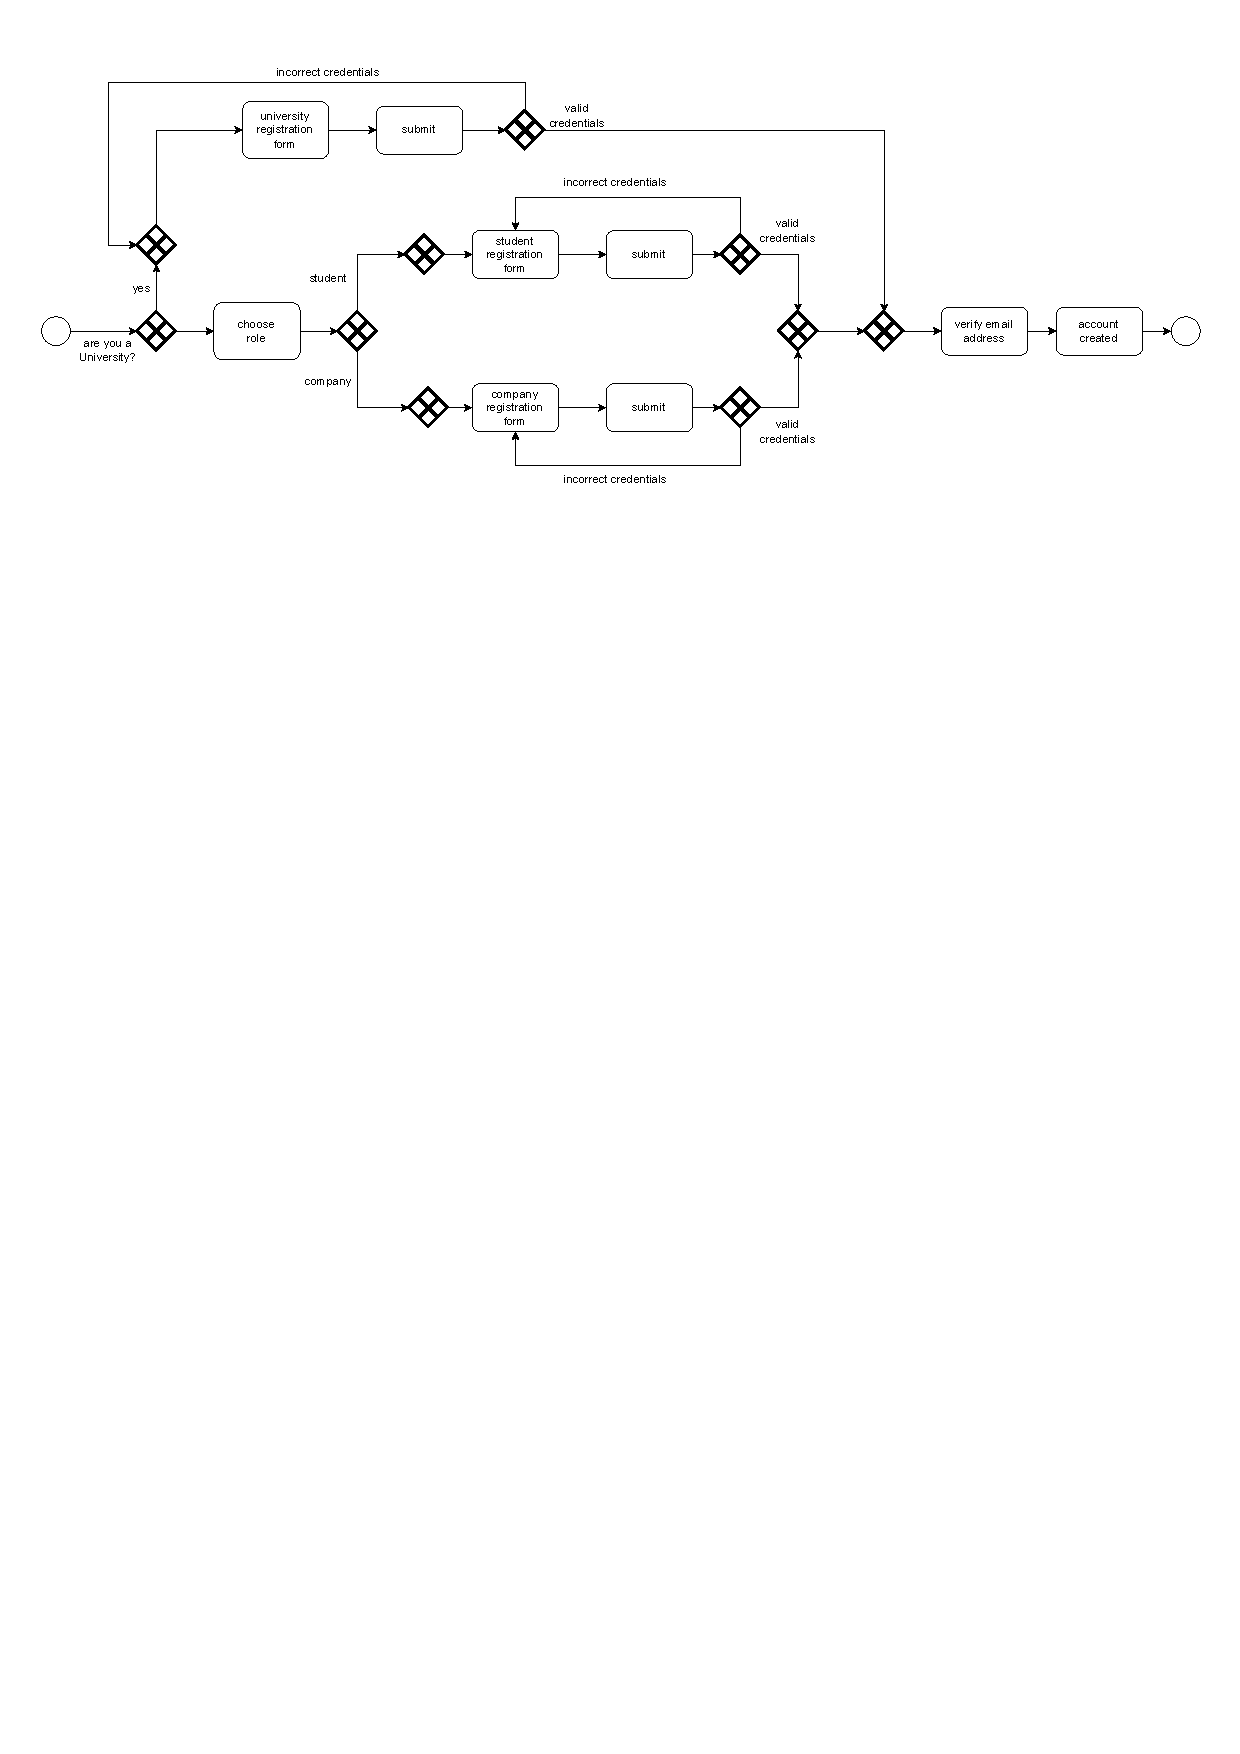
\includegraphics[width=\linewidth]{Images/StateDiagram/SignUp.pdf}
        \caption{Sign Up State Diagram.}
        \label{fig:sign_up_state_diag}%
    \end{center}
\end{figure}

\newpage

\paragraph{Log In:} The login process begins when an existing user 
  opens the web page. The guest is prompted to enter their 
  registered email or username, along with their password.
  If the credentials are invalid, the system shows an error message and
  the user is asked to re-enter the information. If the credentials are
  successfully verified, the system checks if the user's email has been
  previously verified. If the email verification step was skipped, the guest is prompted to verify their email before proceeding. Upon successful verification 
  of all login details, the user is granted access to their dashboard.

\begin{figure}[H]
    \begin{center}
        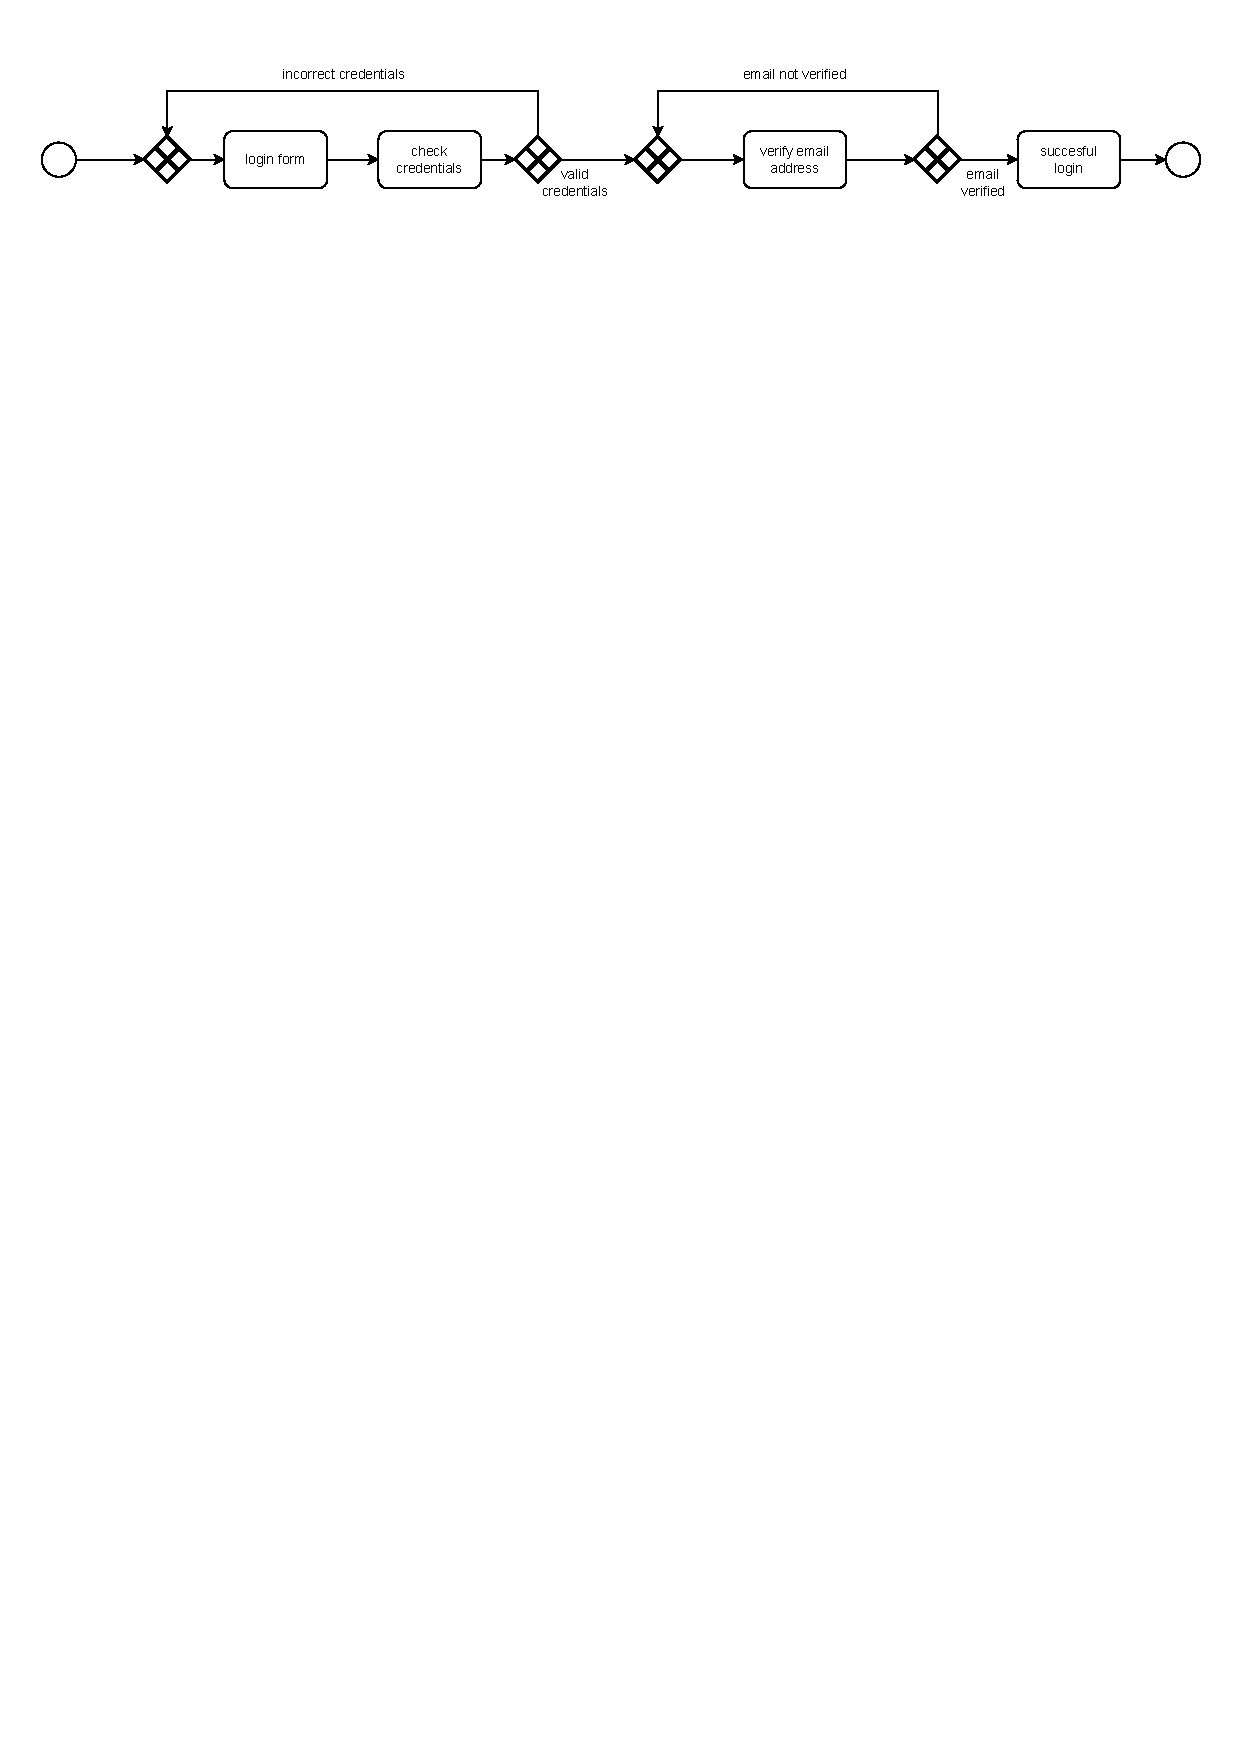
\includegraphics[width=\linewidth]{Images/StateDiagram/Login.pdf}
        \caption{Log In State Diagram.}
        \label{fig:log_in_state_diag}%
    \end{center}
\end{figure}


\paragraph{Enhance your CV:} The process begins when a student opens his
  profile menu and selects the "Enhance" button near the CV. Upon clicking
  the button, the platform initiates the enhancement process by
  analyzing the student's existing CV using AI algorithms. It identifies 
  areas for improvement, including highlighting key skills, rephrasing
  descriptions and adding meaningful action verbs. Once the analysis is
  complete, the AI generates a set of suggestions and provides a preview
  of the enhanced CV. The student can review the suggested changes and
  manually modify his CV. After finalizing the edits, the student
  uploads the enhanced CV to their profile.

\begin{figure}[H]
    \begin{center}
        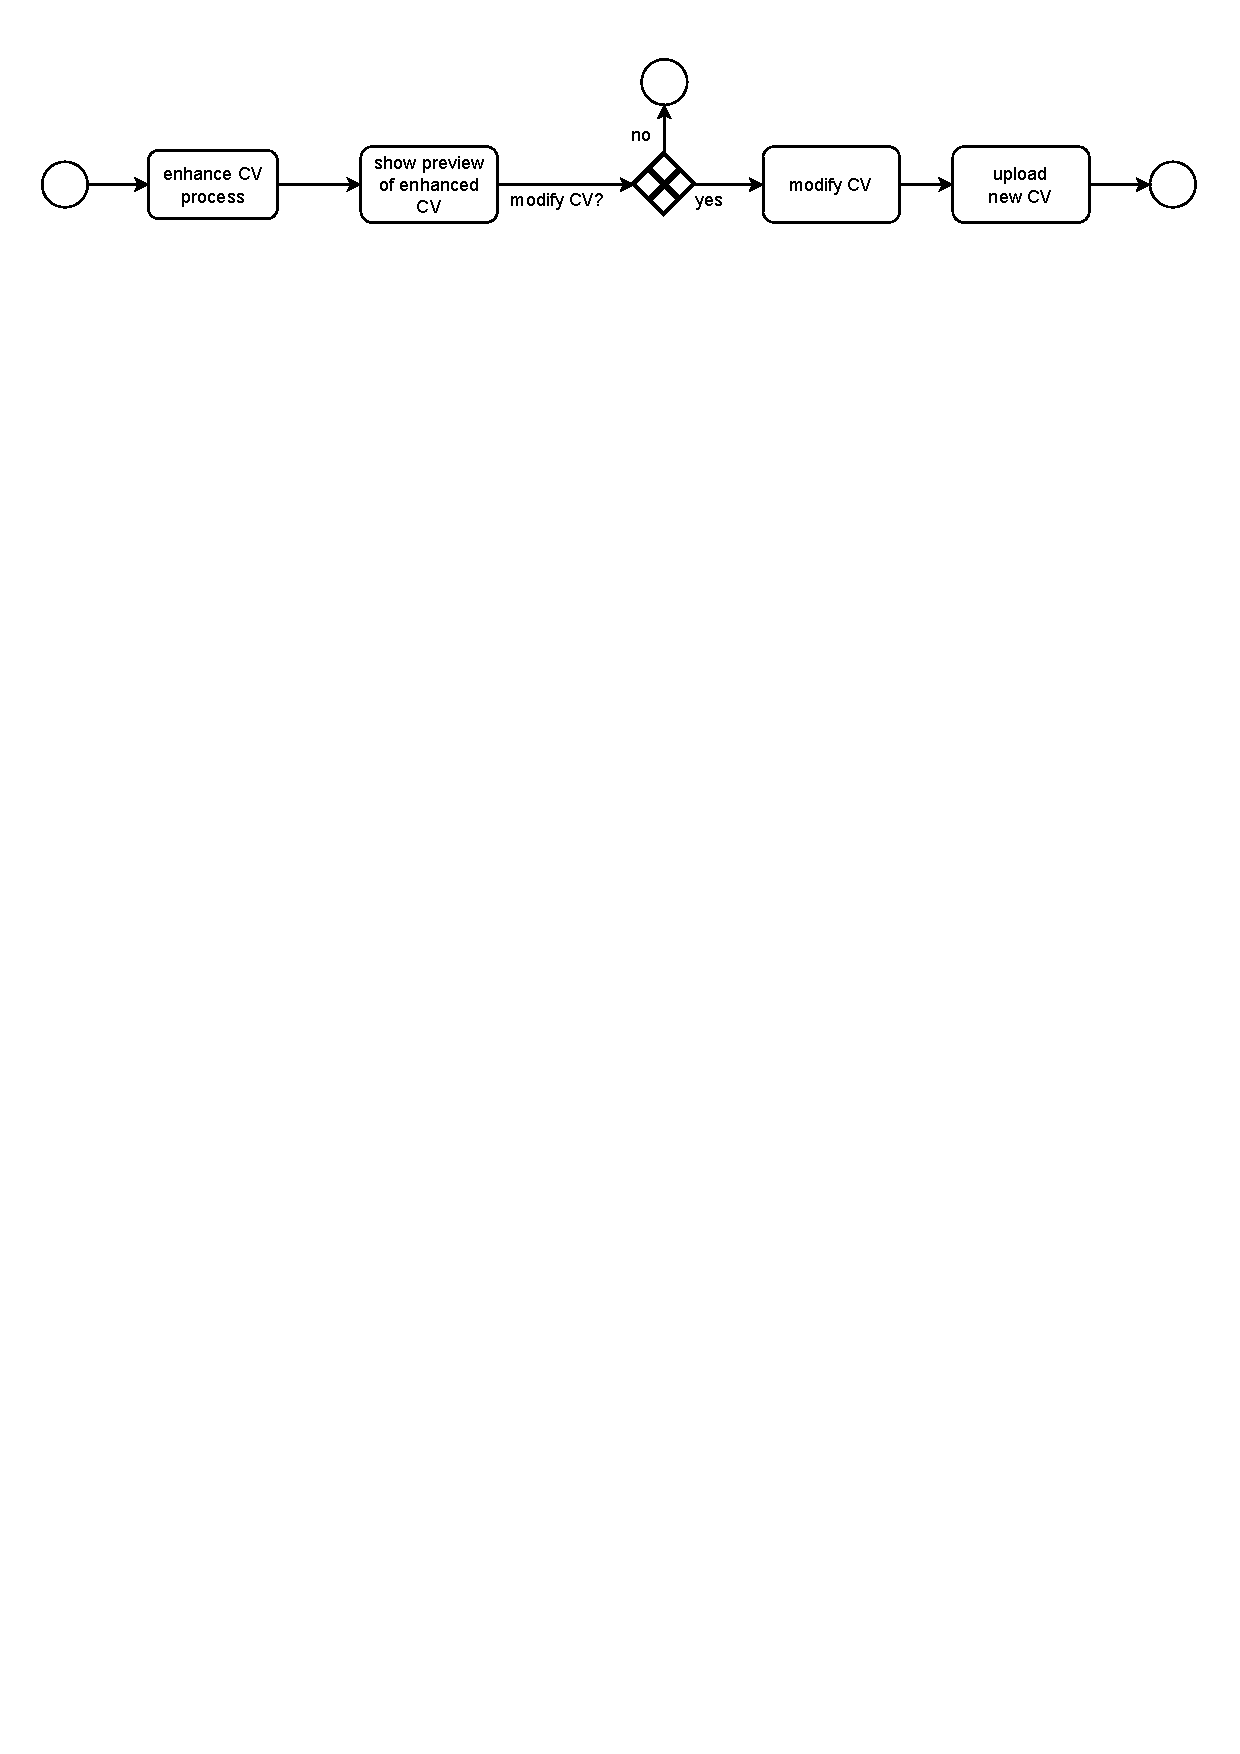
\includegraphics[width=0.9\linewidth]{Images/StateDiagram/EnhanceCV.pdf}
        \caption{Enhance CV State Diagram.}
        \label{fig:enhance_CV_state_diag}%
    \end{center}
\end{figure}

\newpage

\paragraph{Apply for an Internship:} The application process for an
  internship begins when a student clicks on an internship announcement
  that catches their interest. Upon selecting the internship, the
  student is redirected to a detailed view of the internship posting,
  where they can review all relevant information about the job
  description. If the student decides to proceed, they click the "Apply" button. This action inserts the S's profile into the candidates list of the C for the internship that he applied for.

\begin{figure}[H]
    \begin{center}
        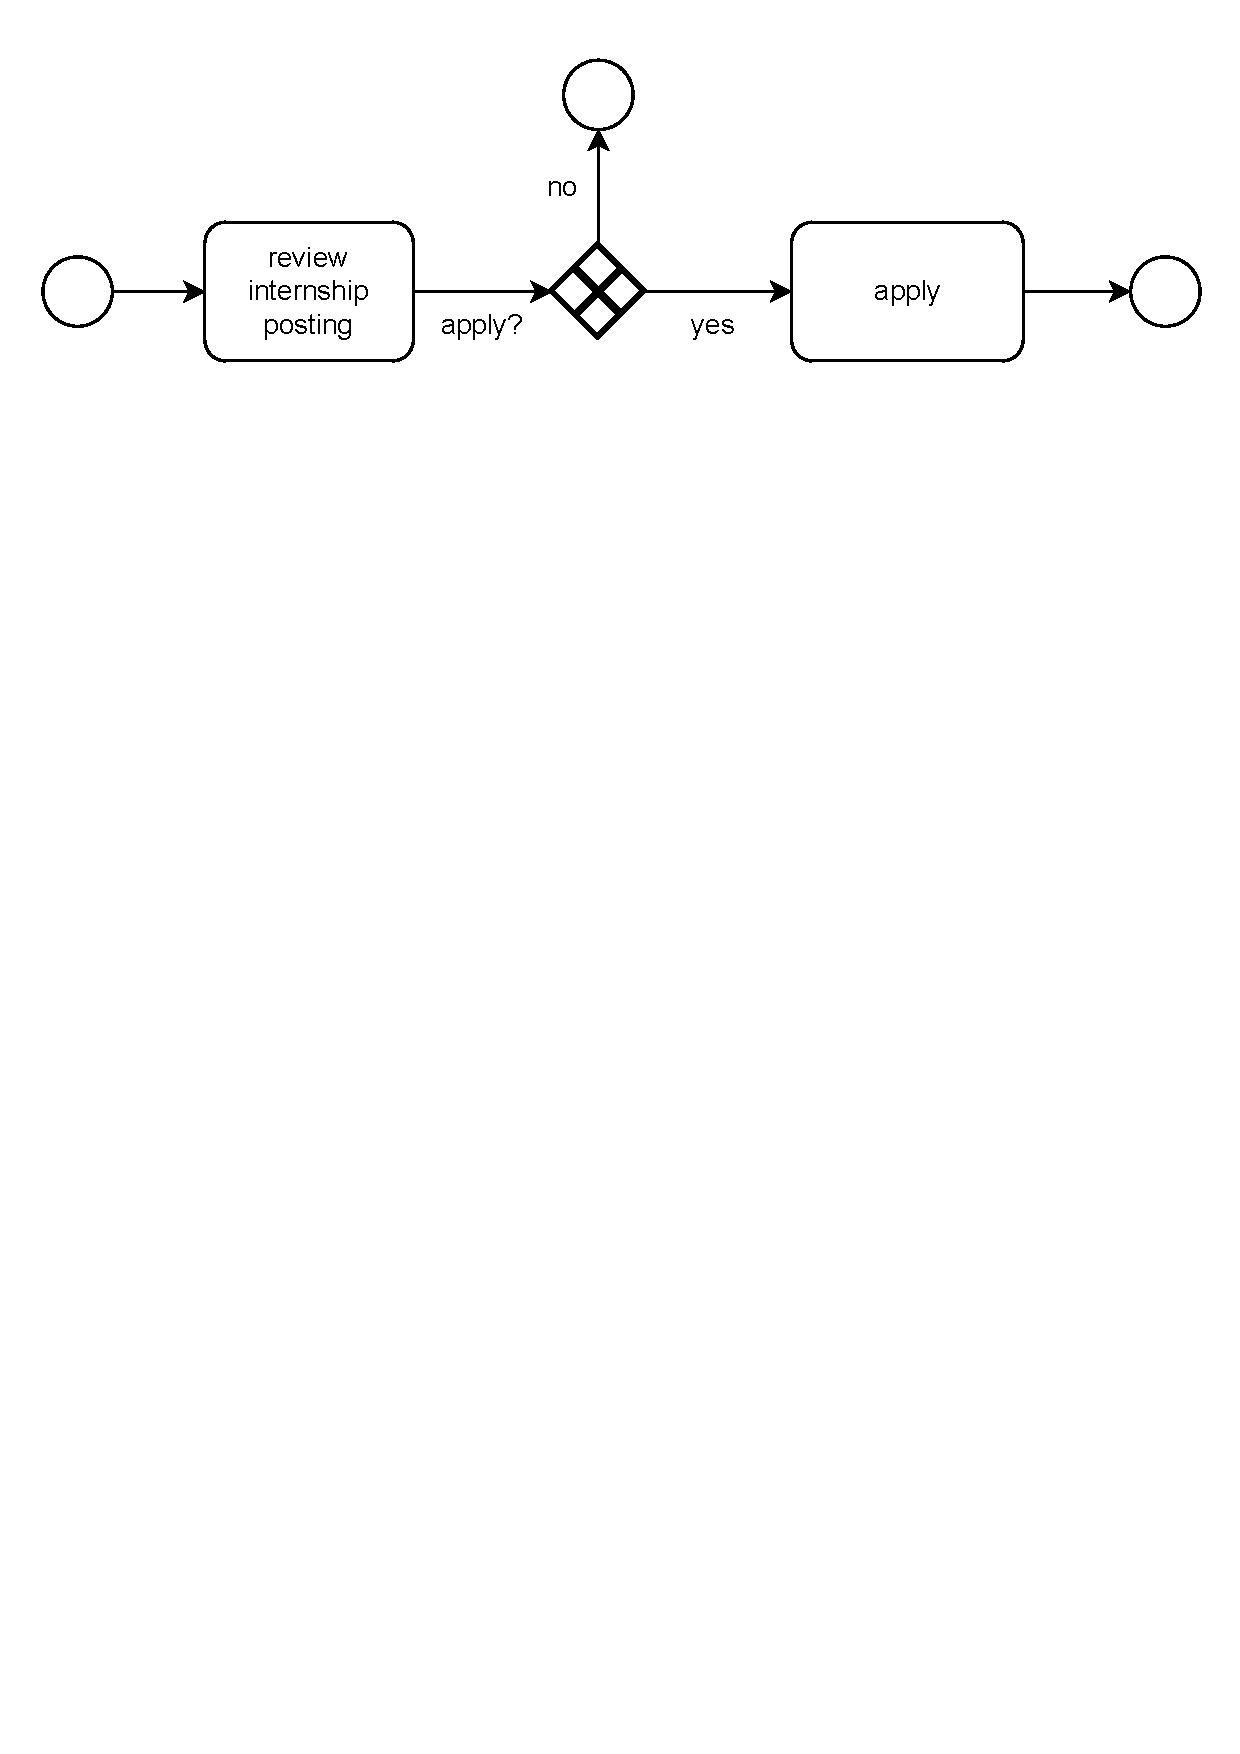
\includegraphics[width=\linewidth]{Images/StateDiagram/Apply.pdf}
        \caption{Apply for an Internship State Diagram.}
        \label{fig:Apply_state_diag}%
    \end{center}
\end{figure}


\paragraph{Require Feedback:} After a user (either a student or a
  company) closes one of the recommended profiles, a pop-up appears
  prompting the user to provide feedback and rating about the
  recommendation. The pop-up includes the question, "Was this recommendation useful?" along with an option to give a rating out of 5 stars and a comment section. This feedback helps the platform improve its recommendation engine, ensuring more accurate matches in the future.

\begin{figure}[H]
    \begin{center}
        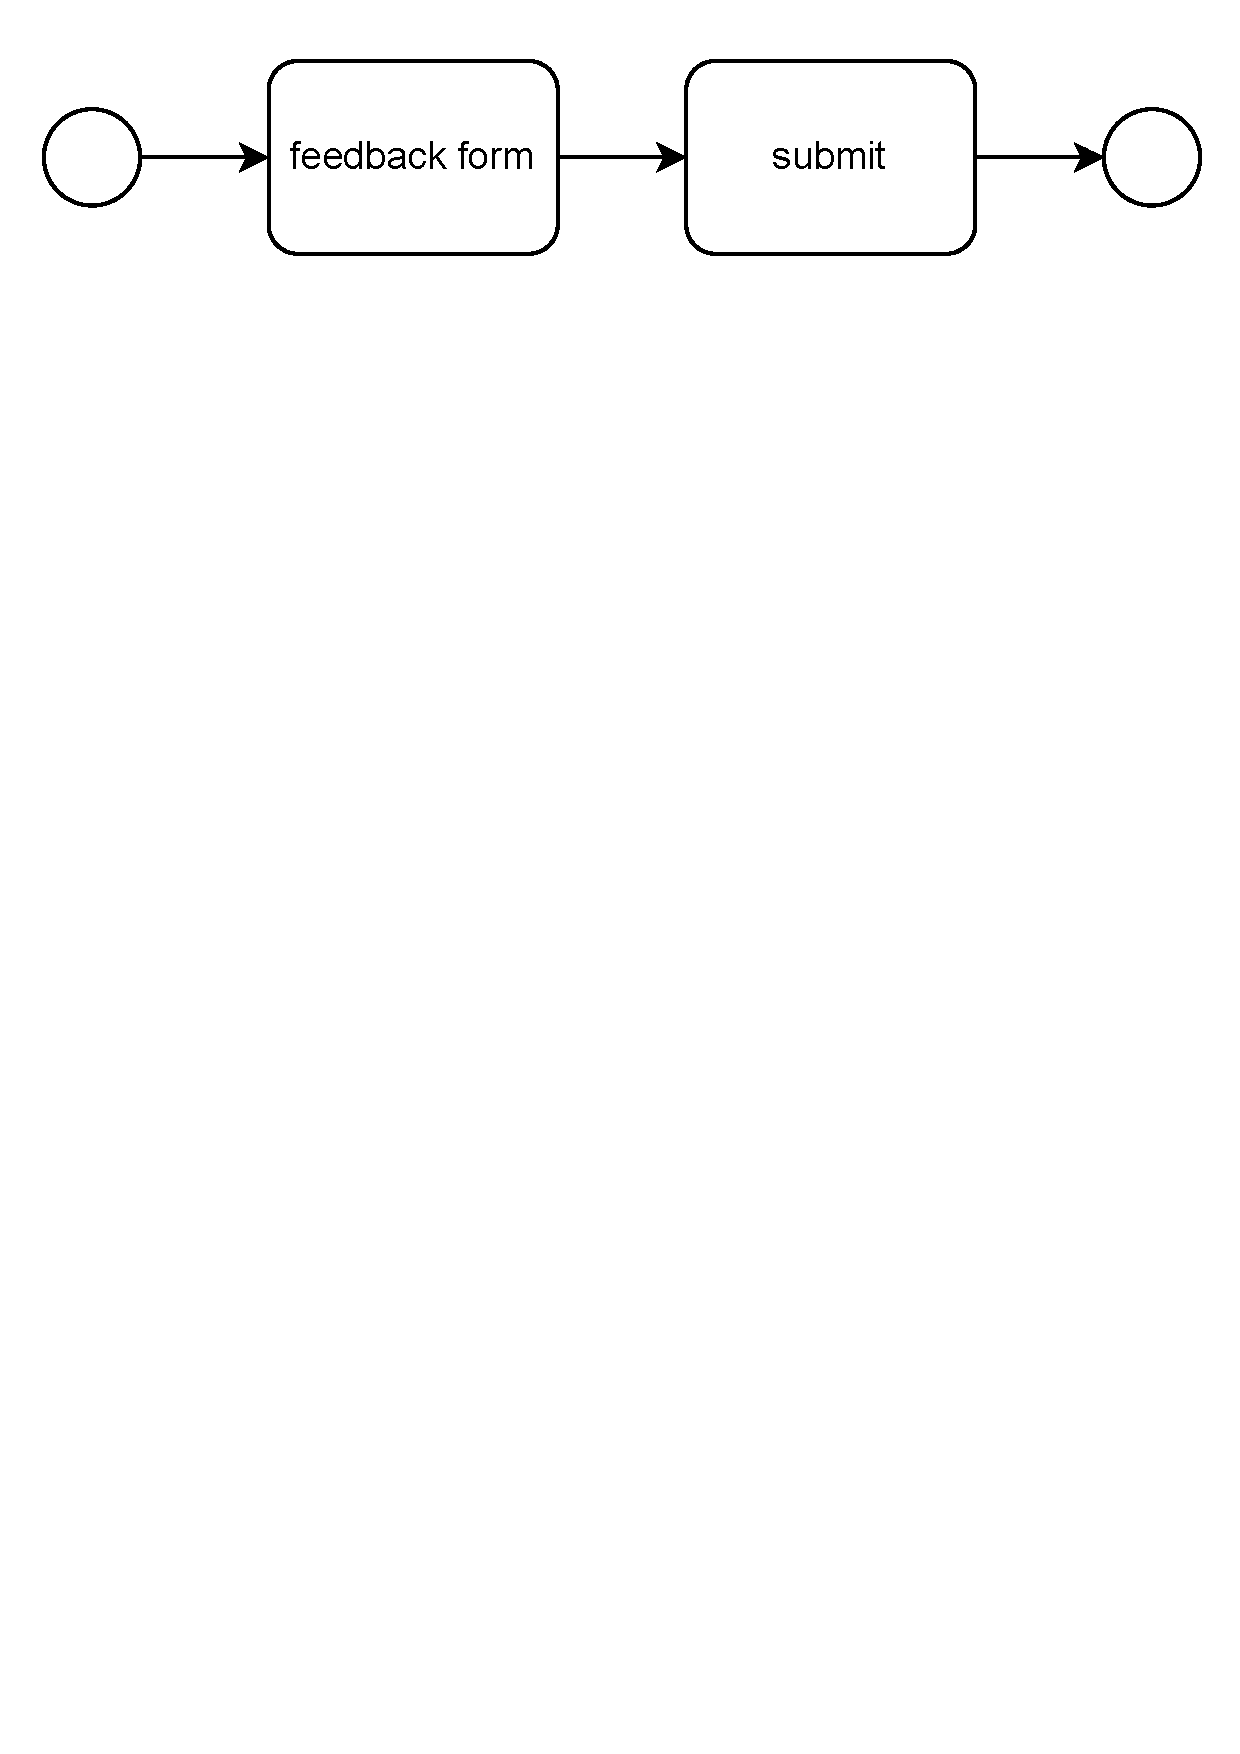
\includegraphics[width=\linewidth]{Images/StateDiagram/RequireFeedback.pdf}
        \caption{Require Feedback State Diagram.}
        \label{fig:req_feedback_state_diag}%
    \end{center}
\end{figure}

\newpage

\paragraph{Insert a new internship and enhance the internship
  description:} After logging in, the company representative selects the
  "Post" button on his dashboard to begin the creation process. The
  system shows a form to input all necessary details about the
  internship. After compiling all the details the representative can also 
  click on the button "Enhance". 
  Upon clicking the button, the platform initiates the enhancement process by analyzing the existing internship
  description using AI algorithms. The AI evaluates various aspects of
  the description, such as clarity, structure, and attractiveness to
  potential candidates. It identifies areas for improvement, such as
  refining the job title, rephrasing the responsibilities and
  requirements for better readability, and highlighting the benefits of
  the internship. Once the analysis is complete, the AI generates a set of
  suggestions. The company representative can review the suggested
  changes and manually modify the insertion.
  Once the representative is satisfied with the details, they submit the internship posting. The system performs validation checks to ensure the following:
  
  -All mandatory fields are completed.
  
  -Data provided is in the correct format (e.g., valid dates for duration, proper email for contact).
  
  After successful validation, the internship is published on the platform and becomes visible to students.

\begin{figure}[H]
    \begin{center}
        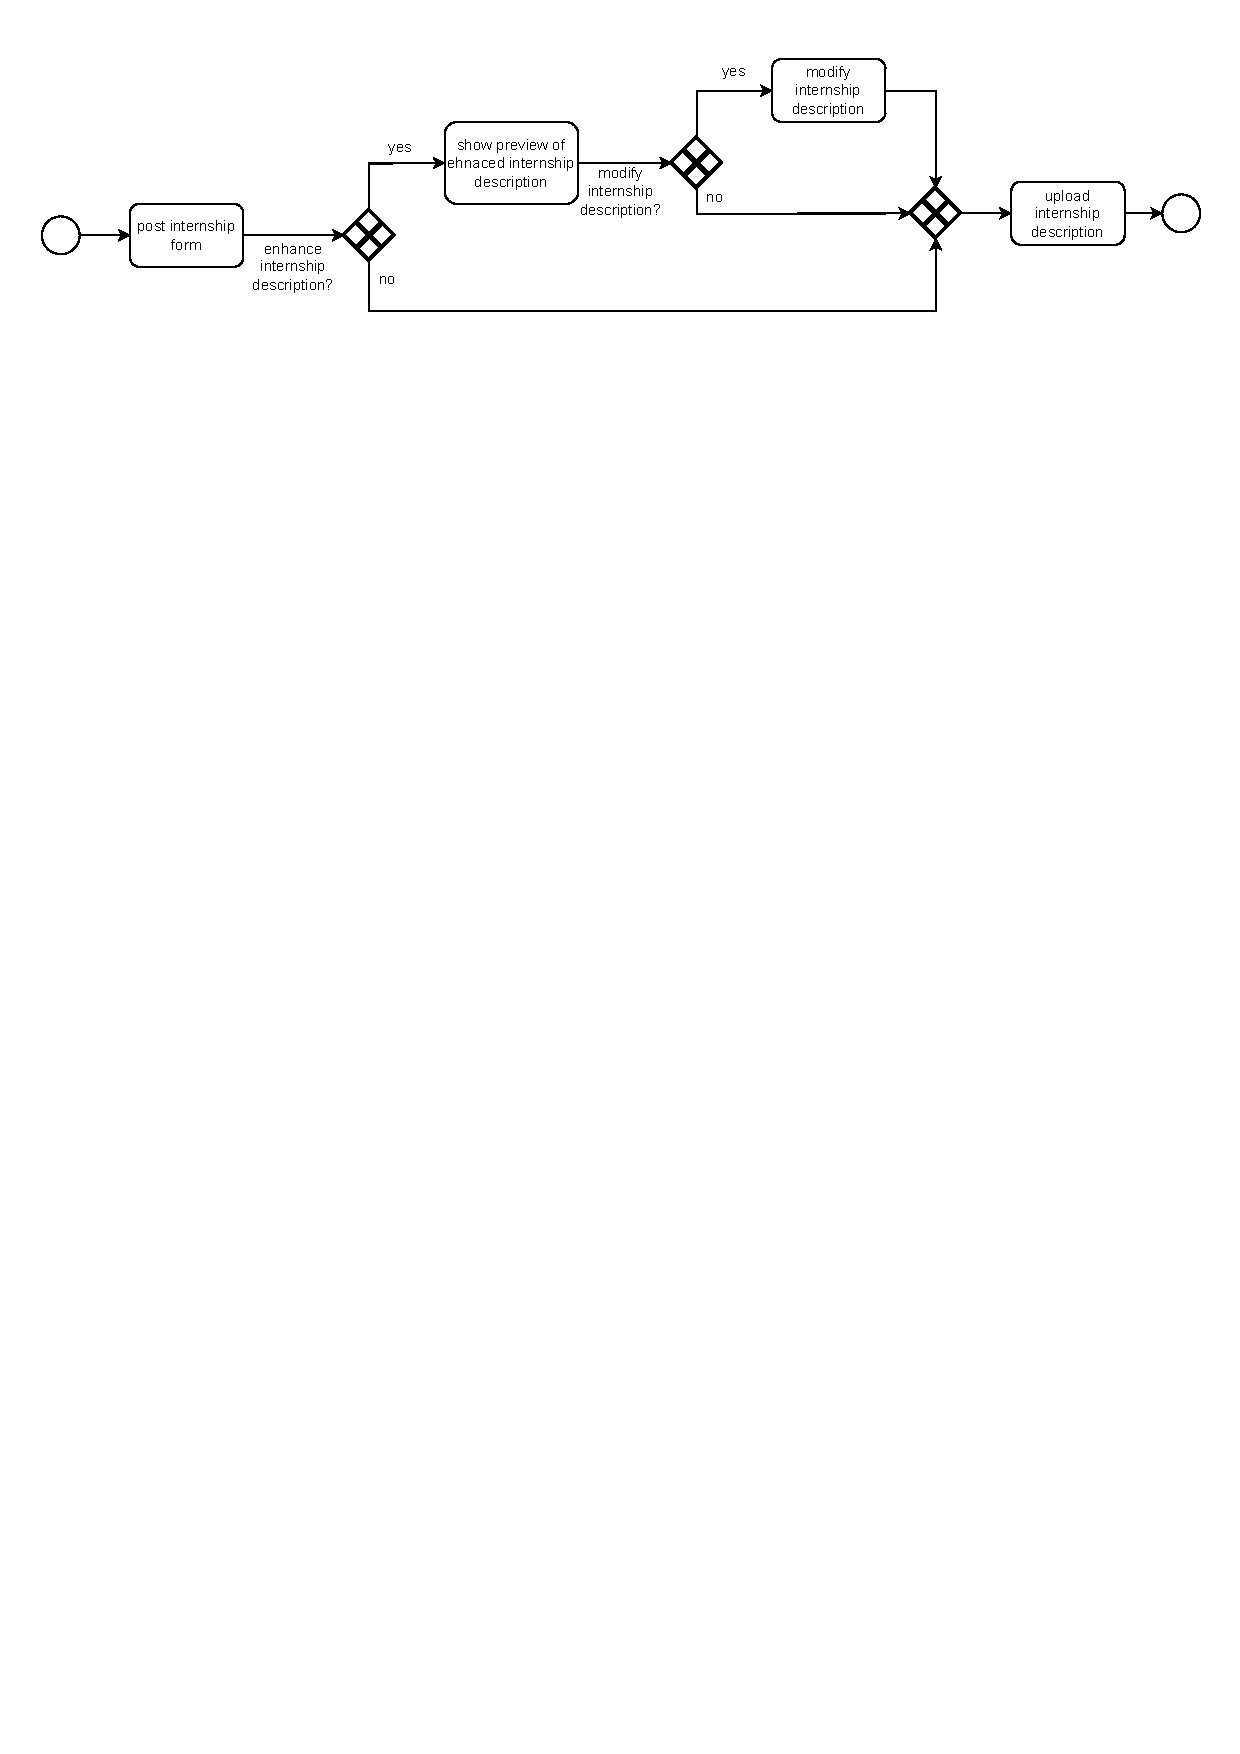
\includegraphics[width=\linewidth]{Images/StateDiagram/Insert&EnhanceInternshipDescription.pdf}
        \caption{Insert and Enhance Internship State Diagram.}
        \label{fig:insert_enhance_intern_state_diag}%
    \end{center}
\end{figure}

\newpage

\paragraph{Selection Process and schedule of interview:} The selection
  process begins when a contact is established between a student and a
  company on the S\&C platform. Once the contact is created, a chat
  opens between the student and the company, allowing them to
  communicate directly. Through the chat, they schedule an interview at
  a mutually convenient time. The company proposes a date and time until
  the student accepts. The event is now added to both the company and
  the student S\&C calendar.
  The interview is conducted separately from the S\&C platform, either in person or using an external virtual meeting tool.

\begin{figure}[H]
    \begin{center}
        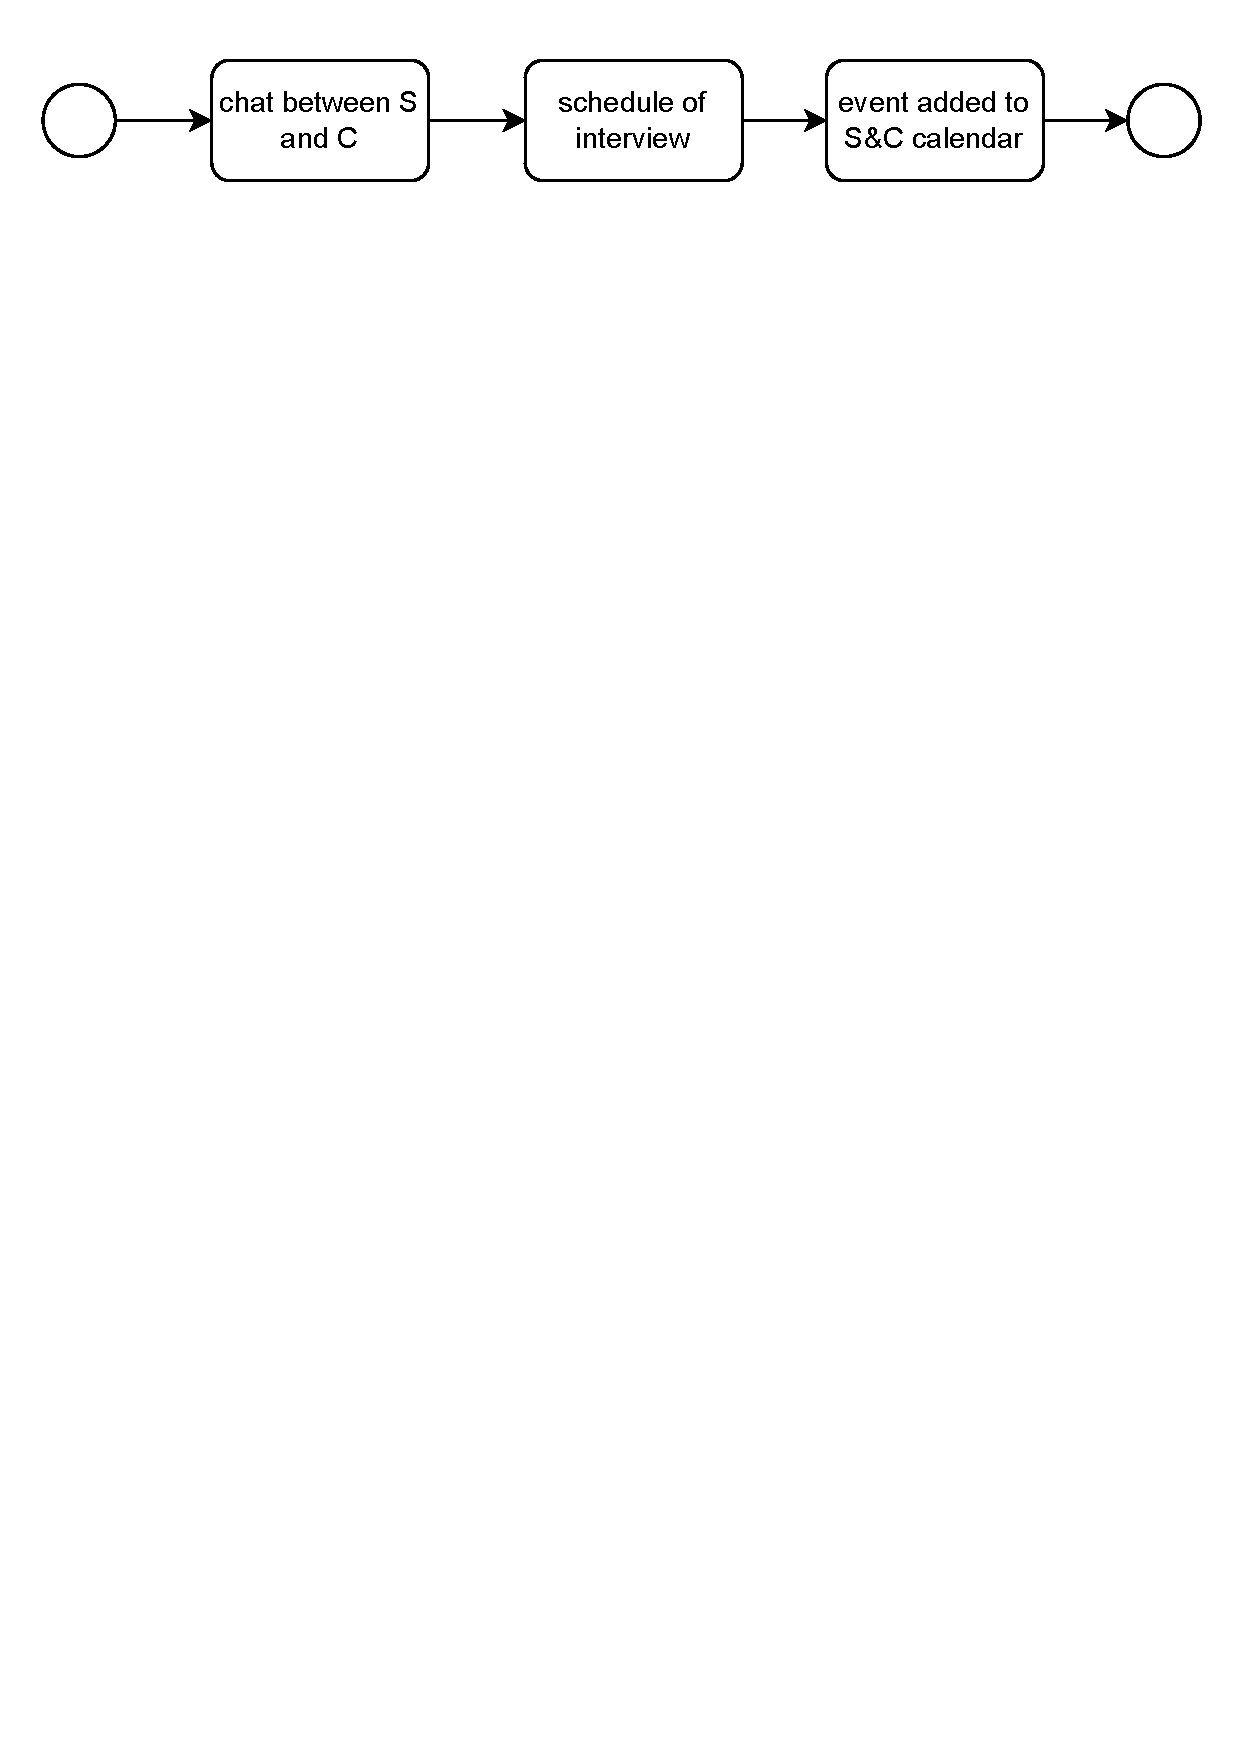
\includegraphics[width=\linewidth]{Images/StateDiagram/SelectionProcess&ScheduleInterview.pdf}
        \caption{Selection and Schedule Interview State Diagram.}
        \label{fig:selection_schedule_interview_state_diag}%
    \end{center}
\end{figure}

\paragraph{Finalizing Process:} The interview was successful and the
  company proposes an internship offer through chat, specifying start
  and end date. Now the student has to make a decision, he can accept or
  refuse through the chat. If the student accepts the event is added to
  the S\&C calendar.

\begin{figure}[H]
    \begin{center}
        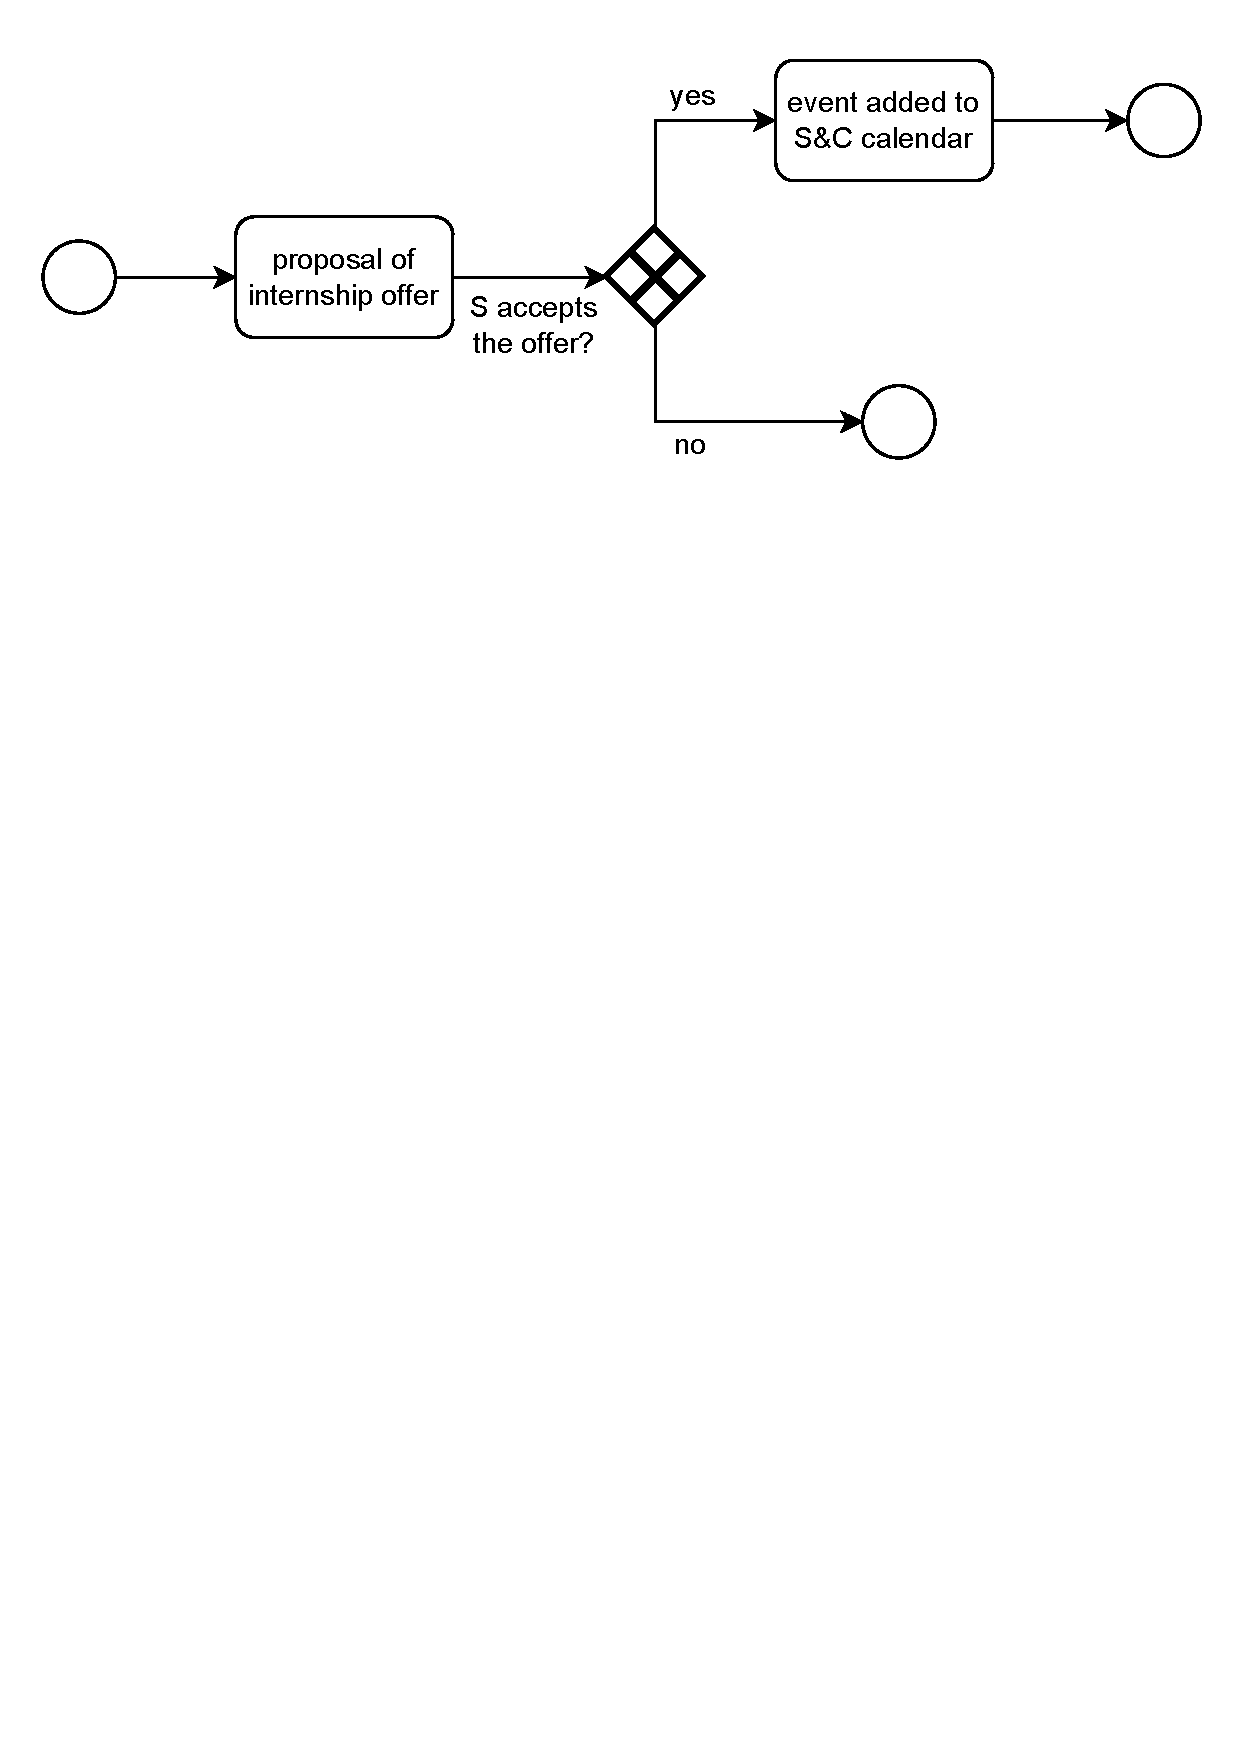
\includegraphics[width=\linewidth]{Images/StateDiagram/FinalizingProcess.pdf}
        \caption{Finalizing Process State Diagram.}
        \label{fig:finalizing_process_state_diag}%
    \end{center}
\end{figure}

\newpage

\paragraph{Report a Problem:} During the internship, either the student
  or the company may encounter an issue that needs to be addressed. To
  report a problem, they can log into the S\&C platform and open the
  chat related to the internship. Here they can click the `Help' button
  and then "Report a Problem". This action opens a form where the user can describe the nature of the
  issue in detail, providing all necessary information. Once the complaint
  is submitted, the event is added to the S\&C calendar, and an email is
  automatically sent to the student's university, alerting them to the problem.

\begin{figure}[H]
    \begin{center}
        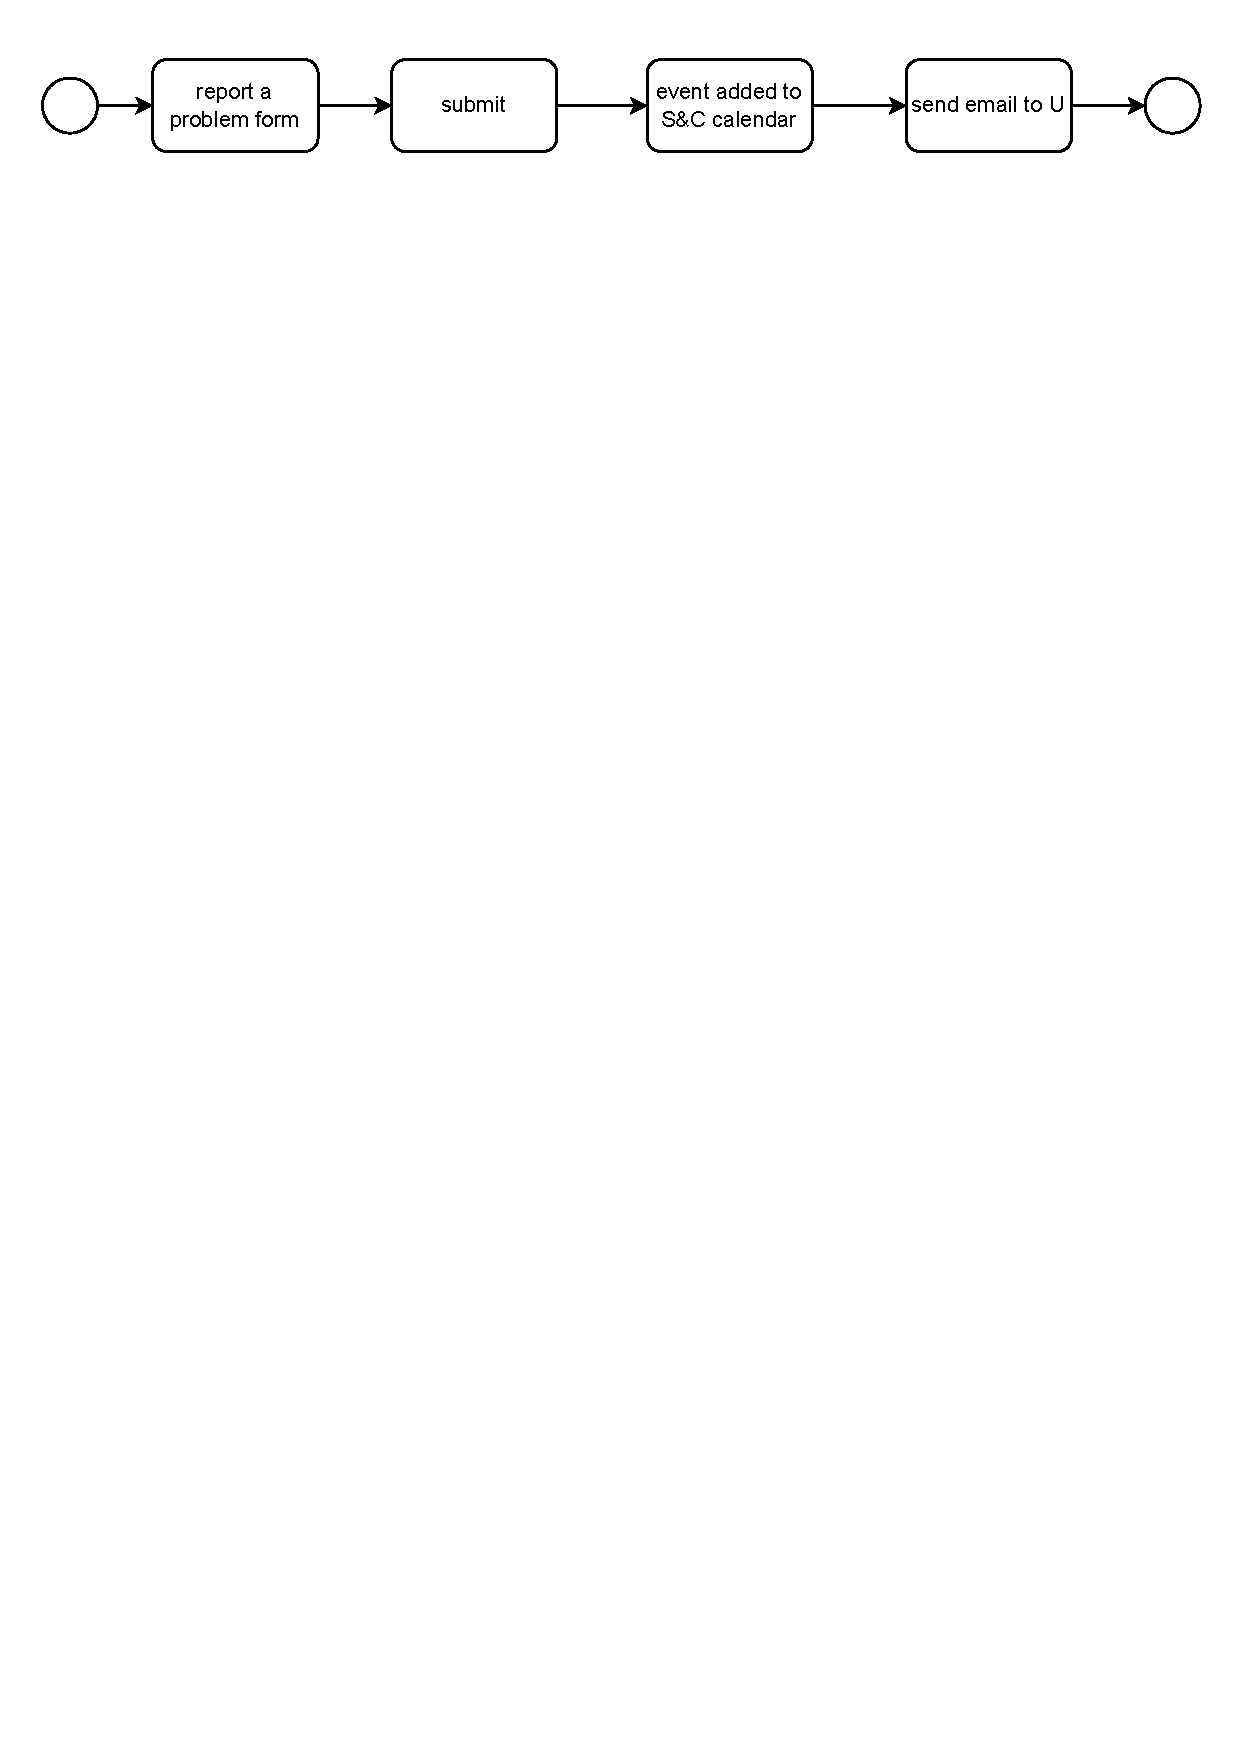
\includegraphics[width=\linewidth]{Images/StateDiagram/ReportProbelm.pdf}
        \caption{Report Problem State Diagram.}
        \label{fig:report_problem_state_diag}%
    \end{center}
\end{figure}

\paragraph{Interrupt Internship:} If the university receives an email
  about a problem reported during an internship, they can log into the
  S\&C platform to review the issue in detail. After evaluating the
  complaint, if the university determines that the situation warrants
  action, they can click on the "Interrupt Internship" button.
  This action terminates the internship between the student and the
  company, ensuring the well-being of the involved parties and addressing
  serious concerns effectively.

\begin{figure}[H]
    \begin{center}
        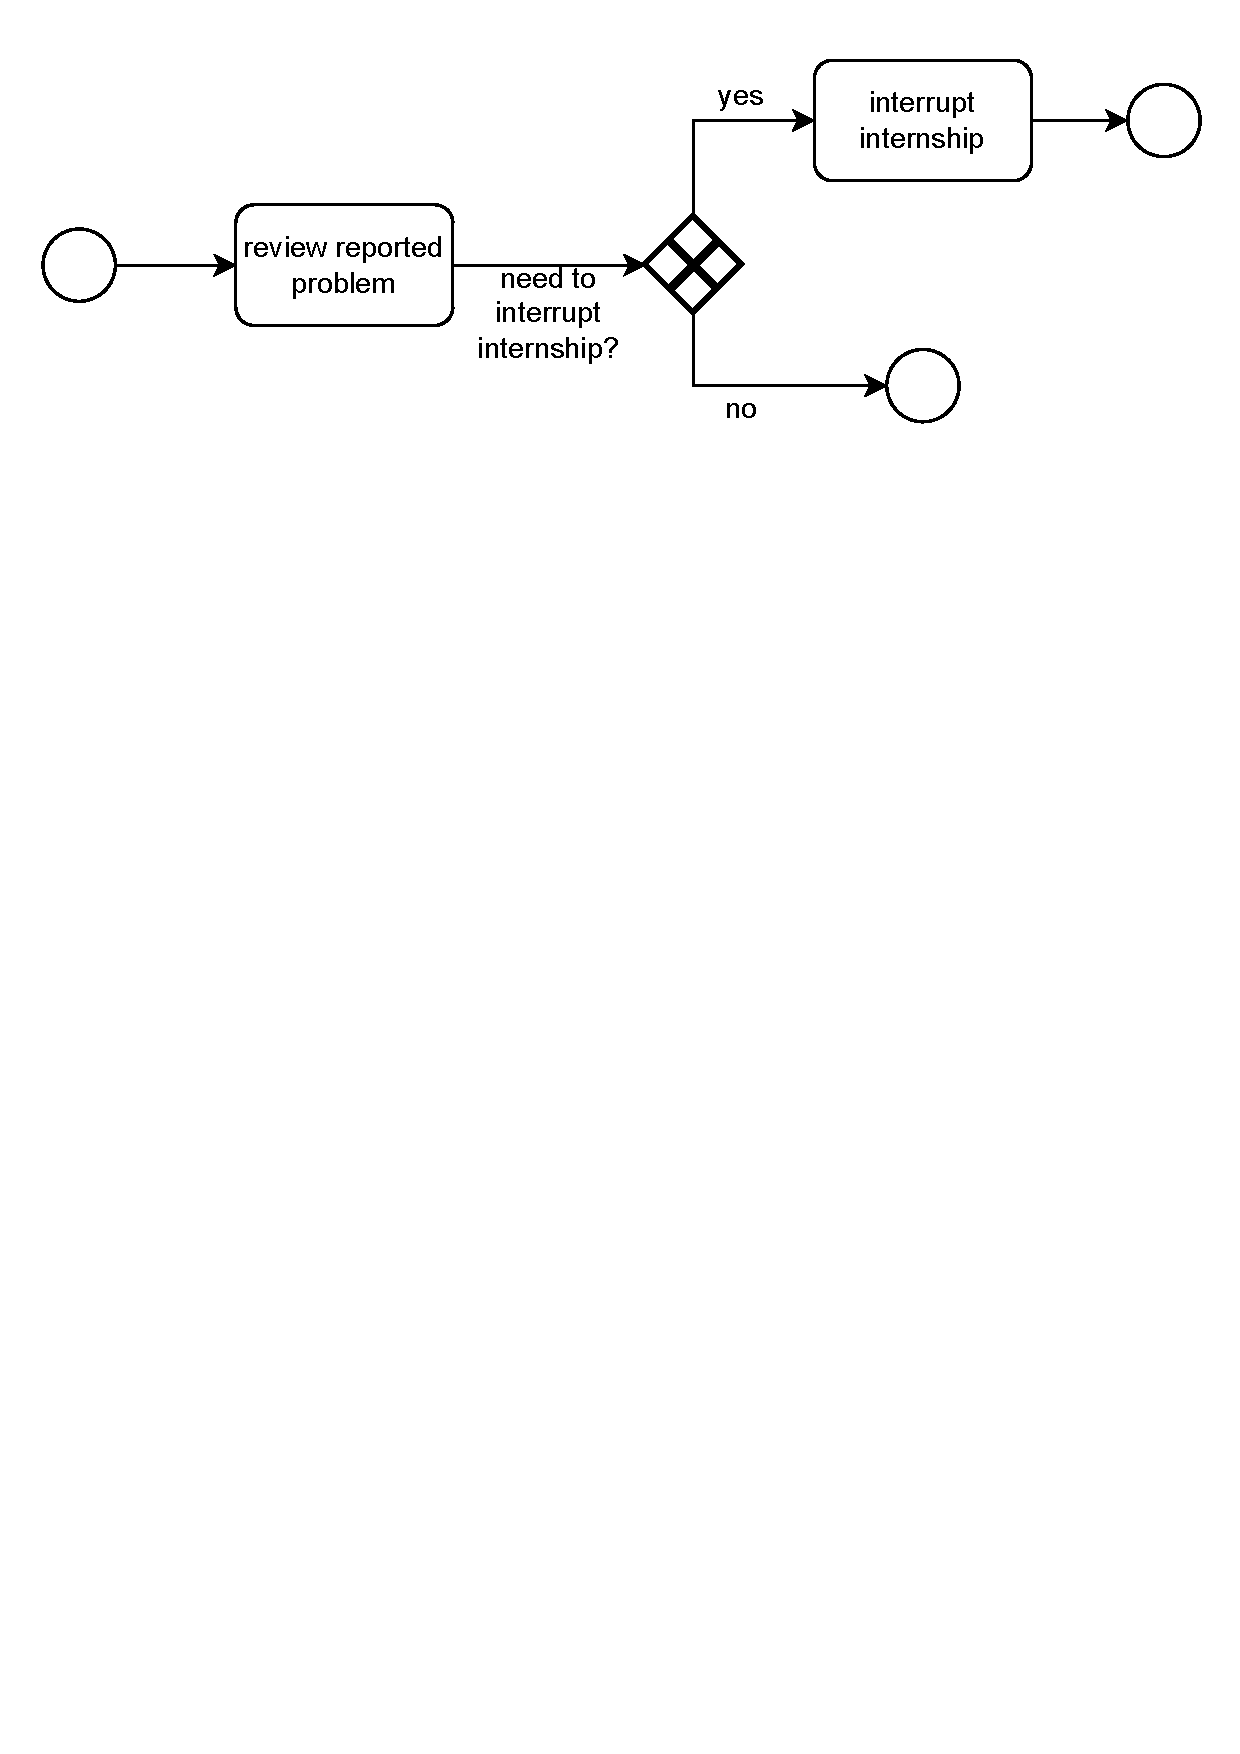
\includegraphics[width=\linewidth]{Images/StateDiagram/InterruptInternship.pdf}
        \caption{Interrupt Internship State Diagram.}
        \label{fig:interrupt_intern_state_diag}%
    \end{center}
\end{figure}

\newpage

\section{Product functions}
\label{sec:product_functions}%

Here is a summary of the main functions of the S\&C system:

\textbf{Sign Up:} The guest begins by selecting the correct category then by clicking the "Sign Up" button, a corresponding form is generated. Then fills out the form by providing the necessary information. A confirmation mail is required to complete the process.

\textbf{Login:} The guest, independently by his category, signs in after
typing his email/username and password in the login form and clicking
the "Login" button.

\textbf{Modify your profile:} The S, C can modify his personal profile
information, such as personal data, profile image, password, email,
username.

\textbf{Enhance the CV}: The S can improve his CV on his
profile's page by clicking the "Enhance" button thanks
to suggestions given by the system.

\textbf{Recommend internships:} The S can look for an internship in the
recommendation's section made by the system.

\textbf{Surf through available internships}: The S can surf through the
search bar on the main page and look for the most pertinent insertion.

\textbf{Ask feedback/suggestions/rating:} The S, C submits feedback,
suggestions and rating about the recommended proposal, when requested.

\textbf{Notify about new internship:} The S is notified when an
internship, considered relevant for him, is found by the system.

\textbf{Notify about new possible candidates:} The C, after submitting
an insertion, is notified when the system finds a relevant match.

\textbf{Submit an internship's insertion:} The C can submit an
internship insertion clicking on "Post" button, by
filling in all the details needed.

\textbf{Improve insertion:} The C can enhance his insertion thanks to
suggestions given by the system, clicking on "Enhance" on the
insertion's page.

\textbf{Apply for an internship:} The S can apply for a preferred
internship, by clicking on "Apply" button on the insertion page.

\textbf{Accept a candidate:} The C can accept one of the candidates that
made an application.

\textbf{Contact a recommended student:} The C can contact one of the
proposed candidates by the recommendation system.

\textbf{Accept a company:} The S can accept a company after being
contacted

\textbf{Create a chat/manage interviews:} After a successful match
between the C and the S, a chat is established in order to manage the
next steps.

\textbf{Sending a contract proposal:} After a successful interview, the C
sends a contract proposal through the chat.

\textbf{Accept/refuse a contract proposal:} After receiving a contract
proposal, the S can decide to accept or refuse the contract through the
chat.

\textbf{Submit Information:} The S,C can submit information about
ongoing internships through the chat.

\textbf{Submit Complaint:} The S, C can submit
complaints/problems during the internship period through the chat.

\textbf{Monitor Internship:} The U can monitor
complaints/information submitted by both parties in its
dashboard.

\textbf{Interrupt Internship:} The U can interrupt an internship if
necessary.

\textbf{Review S\&C calendar:} The C and S can review their personal
events through the S\&C calendar.


\section{User characteristic}
\label{sec:User_characteristic}%

There are two main users S,C and one side U.
Here we have a summary of users characteristics and needs:

\begin{itemize}
\item
  The \textbf{Student}, would like to look for a suitable
  internship opportunity that aligns with his interests. He needs
  guidance in identifying the most relevant offers and support
  throughout the application process. Furthermore, he would like to 
  communicate easily with the company and with the university, 
  in order to address any potential issues.
\end{itemize}

\begin{itemize}
\item
  The \textbf{Company} seeks to efficiently recruit qualified students for new positions, monitor candidates during hiring, and track internship progress. It aims to address student requests and maintain clear communication with both students and their universities to resolve any issues promptly.
\end{itemize}

\begin{itemize}
\item
  The \textbf{University} would like to manage its students during the internship
  period and to intervene promptly when necessary.
\end{itemize}


\section{Assumptions, dependencies and constraints}
\label{sec:assumptions_dependencies_constraints}%

The following assumptions are made for the domain. They represent
foundational expectations and conditions that the S\&C platform will
take for granted. These assumptions define the operational environment
and set the context for the system's design and functionality. They must
be validated to ensure correct platform behavior and a common
understanding of the factors influencing the platform's success.

\newcounter{d}
\setcounter{d}{1}
\newcommand{\cd}{\thed\stepcounter{d}}

\textbf{[D\cd]:} S must be enrolled in a U.

\textbf{[D\cd]:} The related U should be already registered when the S signs up.

\textbf{[D\cd]:} S should already have a valid CV to be uploaded.

\textbf{[D\cd]:} S' CV should be a PDF document.

\textbf{[D\cd]:} The User can easily access his eMail provider.

\textbf{[D\cd]:} S,C provide accurate and truthful information in their
profiles, CVs, and internship description.

\textbf{[D\cd]:} U are willing and able to use the S\&C platform to monitor
internship statuses, address complaints, and respond to student or
company feedback as needed.

\textbf{[D\cd]:} C on the platform are assumed to be legitimate and offer
genuine internships, operating legally and ethically without
verification by S\&C.

\textbf{[D\cd]:} The S\&C recommendation engine achieves high accuracy when S
and C provide detailed, complete, and accurate information in their CVs
and job descriptions.

\textbf{[D\cd]:} The AI system integrated into the S\&C platform effectively
enhances students' CVs and companies' internship postings, 
providing accurate and useful suggestions to improve the matching process.

\textbf{[D\cd]:} The eMail provider functions reliably, ensuring that all
emails, including verification and notification messages, are
successfully delivered to the intended recipients.

\textbf{[D\cd]:} Students and companies are committed to the internship process
and will engage with features such as scheduling interviews and
responding to feedback.

\textbf{[D\cd]:} Companies must clearly communicate interview requirements
(e.g., time, format, platform) to students during scheduling.

\textbf{[D\cd]:} Interviews must be conducted either in person or via secure
external tools, with students and companies responsible for ensuring
their availability and functionality.